
\clearpage
\section{Die Übersicht über Geschäfte bewahren}

Der Teil 'Geschäfte' des CUBE PA unterstützt das Führen eines strukturierten Projektjournals. Das Projektjournal besteht aus einer Sammlung von Geschäften, die ihrerseits in Teilgeschäfte unterteilt sind. Die Anzahl Teilgeschäfte ist unbeschränkt. Für jedes Teilgeschäft besteht im CUBE PA eine Chronologie, die mit dem jüngsten Eintrag zuoberst angezeigt wird.

\vspace{\baselineskip}

Die Philosophie hinter der Struktur von Geschäften und Teilgeschäften lässt sich durch folgendes Beispiel erklären: Sie werden zum Direktor befördert und müssen sich deshalb standesgemäss einkleiden. Das Geschäft 'Businessanzüge kaufen' lässt sich in eine Reihe von Teilgeschäften aufteilen: zur Farbberatung gehen,
Marktforschung bei den wichtigsten Online-Angeboten betreiben, Anzüge kaufen, Hemden kaufen, Schuhe kaufen, etc. Sobald alle Teilgeschäfte abgeschlossen sind, ist auch das Geschäft abgeschlossen.

\vspace{\baselineskip}

Innerhalb jedes Teilgeschäfts lässt sich die Historie in Form von Einträgen aufzeichnen. Einträge entsprechen im Grunde genommen den Zeilen einer Excel-Tabelle. Die Idee ist, alle für das Projektjournal relevanten Vorgänge in Form von Einträgen zu erfassen. Der CUBE PA stellt die Einträge chronologisch dar, mit den jüngsten Einträgen zuoberst.

\subsection{Ein Geschäft erfassen}

\begin{wrapfigure}[1]{l}{6.5cm}   % [x] Wie manche Zeile soll sich um die Grafik "brechen"
  \vspace{-35pt}      % Grundwert war 20; mit 30 schön oben beim Text ausgerichtet
  \begin{center}
    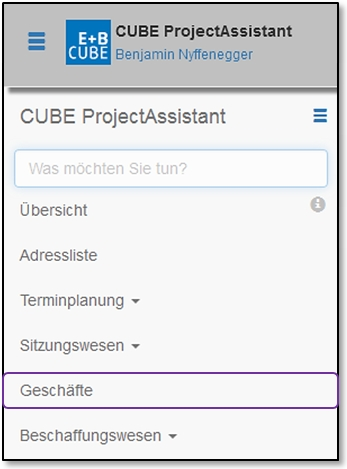
\includegraphics[width=1\linewidth]{../chapters/06_Geschaefte/pictures/6-1_Menu_Geschaefte.jpg}
  \end{center}
  \vspace{-20pt}
  \caption{Geschäfte und Verträge organisieren}
  \vspace{-10pt}
\end{wrapfigure}

Wählen Sie im Menü links den Punkt 'Geschäfte'. \\

% \vspace{6cm}
\pagebreak

Daraufhin erscheint die Liste der Geschäfte:

%\pagebreak

\begin{figure}[H]
\center{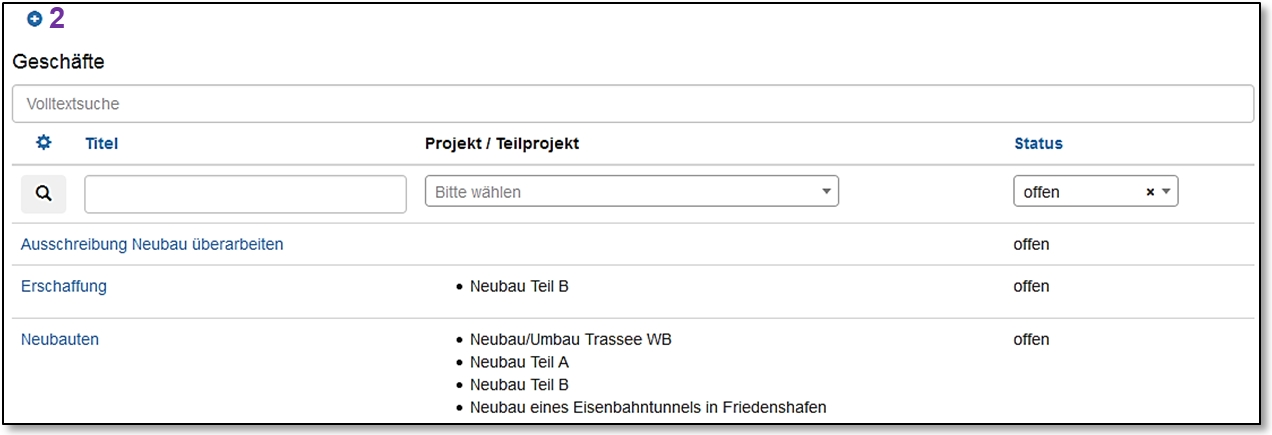
\includegraphics[width=1\linewidth]{../chapters/06_Geschaefte/pictures/6-1_GeschaefteUebersicht.jpg}}
\caption{Übersicht der Geschäfte}
% \label{fig:speciation}
\end{figure}

Klicken Sie auf das Pluszeichen 
\includegraphics[height=12pt]{/Icons/Plussymbol.jpg} \col{(2)} oben links und es erscheint die Maske für das Erfassen eines neuen Geschäfts.

\begin{figure}[H]
\center{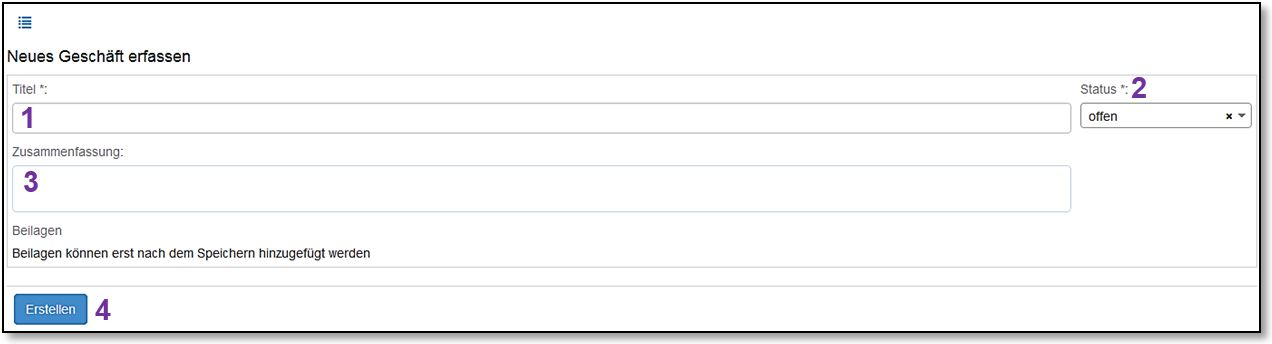
\includegraphics[width=1\linewidth]{../chapters/06_Geschaefte/pictures/6-1_NeueGeschaefteErfassen.jpg}}
\caption{Neue Geschäfte erfassen}
% \label{fig:speciation}
\end{figure}

Mussfelder sind mit einem Stern * markiert.

\begin{itemize}
\item
Titel \col{(1)}: hier geben Sie den Namen des Geschäfts als freien Text ein.
\item 
Status \col{(2)}: Es gibt nur die Stati 'offen' und 'abgeschlossen'. Der erstere ist beim Erstellen eines neuen Geschäfts gesetzt, den letzteren können Sie setzen, wenn das Geschäft erledigt ist.
\item
Zusammenfassung \col{(3)}: Hier schreiben Sie in zwei, drei Zeilen freien Text, um was es beim Geschäft geht.
\end{itemize}

Klicken Sie auf die Schaltfläche 'Erstellen' 
\includegraphics[height=12pt]{/Icons/B_Erstellen.jpg} \col{(4)}. Nun können Sie Beilagen hochladen:

\begin{figure}[H]
\center{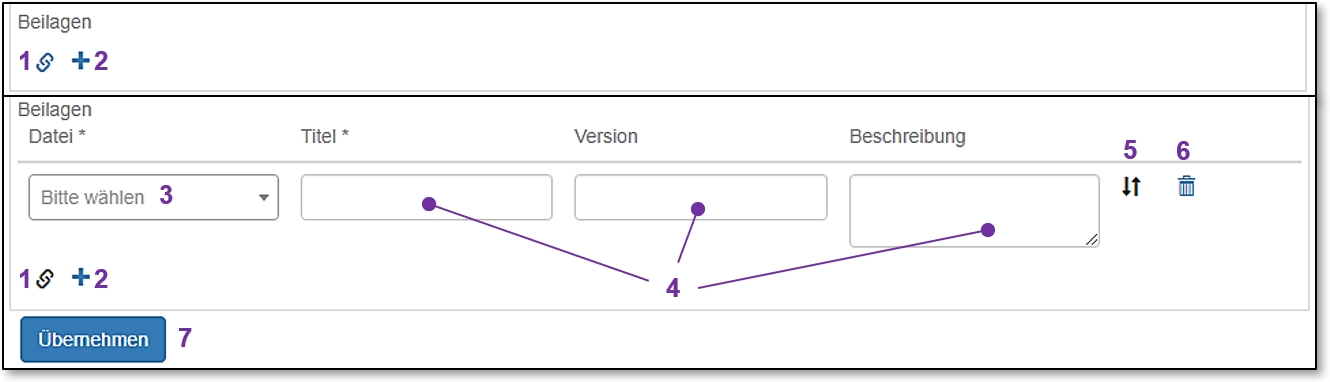
\includegraphics[width=1\linewidth]{../chapters/06_Geschaefte/pictures/6-1_GeschaefteBeilagenHochladen.jpg}}
\caption{Beilagen hochladen}
% \label{fig:speciation}
\end{figure}

\textbf{Anmerkung:} Das Hochladen von Beilagen ist vor allem dazu gedacht, das Erfassen von langen Erklärungen zu vermeiden und dafür auf eine hochgeladene Beilage zu verweisen.

\vspace{\baselineskip}

Soll eine Beilage erfasst werden, klicken Sie entweder auf das Linkzeichen 
\includegraphics[height=12pt]{/Icons/Link.jpg} \col{(1)}, um ein bereits in CUBE PA vorhandenes Dokument zu verknüpfen oder auf das Pluszeichen 
\includegraphics[height=12pt]{/Icons/Pluszeichen.jpg} \col{(2)}, um ein neues Dokument hochzuladen. 

\vspace{\baselineskip}

Wenn Sie auf das Linkzeichen 
\includegraphics[height=12pt]{/Icons/Link.jpg} \col{(1)} klicken, wird das untere Fenster sichtbar und Sie können unter 'Bitte wählen' \col{(3)} eine Datei auswählen, welche bereits in der Dokumentenablage abgelegt wurde. Klicken Sie auf den gewünschten Dokumentennamen, werden Ihnen die verschiedenen Versionen angezeigt und Sie können exakt die benötigte Version verknüpfen. Nun können Sie die Felder 'Titel*' (Pflichtfeld), 'Version' und 'Beschreibung' \col{(4)} anpassen.

\vspace{\baselineskip}

Wenn Sie auf das Pluszeichen 
\includegraphics[height=12pt]{/Icons/Pluszeichen.jpg} \col{(2)} klicken, wird das aus der Dokumentenablage bekannte Dialogfenster zum Hochladen von Dateien geöffnet. Weitere Informationen zum Hochladen finden Sie unter Kapitel \ref{bkm:Ref442769978}.\
Sie können beliebig viele Dokument verpnüpfen \col{(1)} oder hochladen \col{(2)}. Wiederholen Sie dazu obige Schritte. Haben Sie mehrere Beilagen erfasst, können Sie mittels Linksklick auf die vertikalen Pfeilen 
\includegraphics[height=12pt]{/Icons/VertPfeile.jpg} \col{(5)} (halten und verschieben) die Reihenfolge anpassen. Durch einen Klick auf das Mülltonnensymbol 
\includegraphics[height=12pt]{/Icons/Muelltonne.jpg} \col{(6)} werden Beilagen gelöscht.

\vspace{\baselineskip}

Speichern Sie die Beilagen sowie Eingaben mit Klick auf 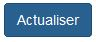
\includegraphics[height=14pt]{/Icons/B_Uebernehmen.jpg} \col{(6)} ab.

% Bishierher

\vspace{\baselineskip}

Sie können so viele Beilagen erfassen wie erforderlich, indem Sie immer wieder auf das Pluszeichen 
\includegraphics[height=12pt]{/Icons/Pluszeichen.jpg} \col{(5)} klicken. Sie können die Reihenfolge der Beilagen ändern, indem Sie mit der linken Maustaste das Symbol mit vertikalen Pfeilen 
\includegraphics[height=12pt]{/Icons/VertPfeile.jpg} \col{(6)} packen und die Zeile verschieben. Durch einen Klick auf das Mülltonnensymbol 
\includegraphics[height=12pt]{/Icons/Muelltonne.jpg} \col{(7)} können Sie eine Beilage löschen.

% bishierher

\subsection{Ein Teilgeschäft erfassen}

Entweder fahren Sie gleich auf demselben Bildschirm weiter wie beim Erfassen von Beilagen zu einem Geschäft, oder Sie steigen wieder über das Menü ein und wählen den Punkt 'Geschäfte'. In der Liste der Geschäfte können Sie das Geschäft suchen, zu dem Sie ein Teilgeschäft erfassen wollen.

\vspace{\baselineskip}

Sie können nun optisch innerhalb der gesamten Liste der Geschäfte suchen oder die Liste filtern. Zum Blättern in der Liste scrollen Sie einfach nach unten, zuunterst sehen Sie Schaltflächen zum Blättern auf eine nächste Seite, oder zum Weiter- oder Zurückblättern.

\begin{center}

\includegraphics[height=16pt]{/Icons/SeitenBlaettern.jpg}
\end{center}

Zum Filtern der Liste stehen Ihnen die Suchfelder in der ersten Zeile zur Verfügung, sowie ein separates Feld für die Volltextsuche \col{(1)}. Im Feld 'Titel' \col{(2)} können Sie freien Text eingeben; im Feld 'Projekt/Teilprojekt' \col{(3)}, sowie im Feld 'Status' \col{(4)} steht jeweils eine Auswahlliste zur Verfügung. Haben Sie die Filterwerte ausgewählt, klicken Sie auf das Lupensymbol 
\includegraphics[height=12pt]{/Icons/Lupe_kl.jpg} \col{(5)} links (oder drücken die 'Enter'-Taste) und die gefilterte Liste erscheint. Alternativ können Sie mittels der Volltextsuche nach Stichworten in der Liste suchen, welche nach Klick auf die Lupe 
\includegraphics[height=12pt]{/Icons/Lupe_kl.jpg} \col{(5)} oder der 'Enter'-Taste ausgeführt wird.

\begin{figure}[H]
\center{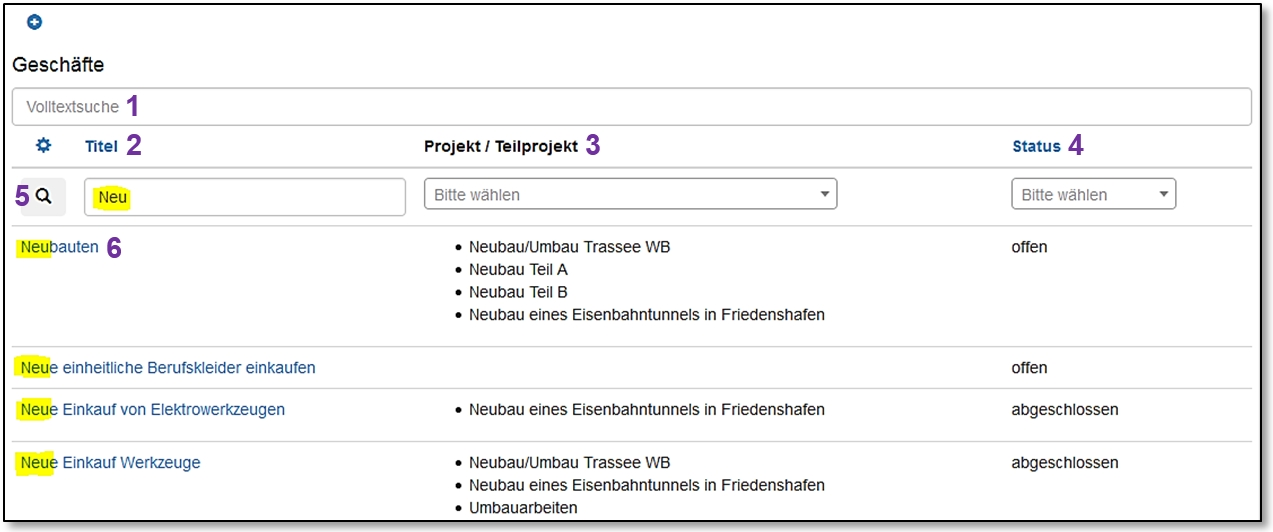
\includegraphics[width=1\linewidth]{../chapters/06_Geschaefte/pictures/6-2_FilterAnwenden.jpg}}
\caption{Der Filter verwenden}
% \label{fig:speciation}
\end{figure}


Haben Sie das relevante Geschäft gefunden, klicken Sie auf den blauen Titeltext des entsprechenden Geschäftes \col{(6)}. Nun erscheint die Maske mit der Übersicht über das Geschäft.

\begin{figure}[H]
\center{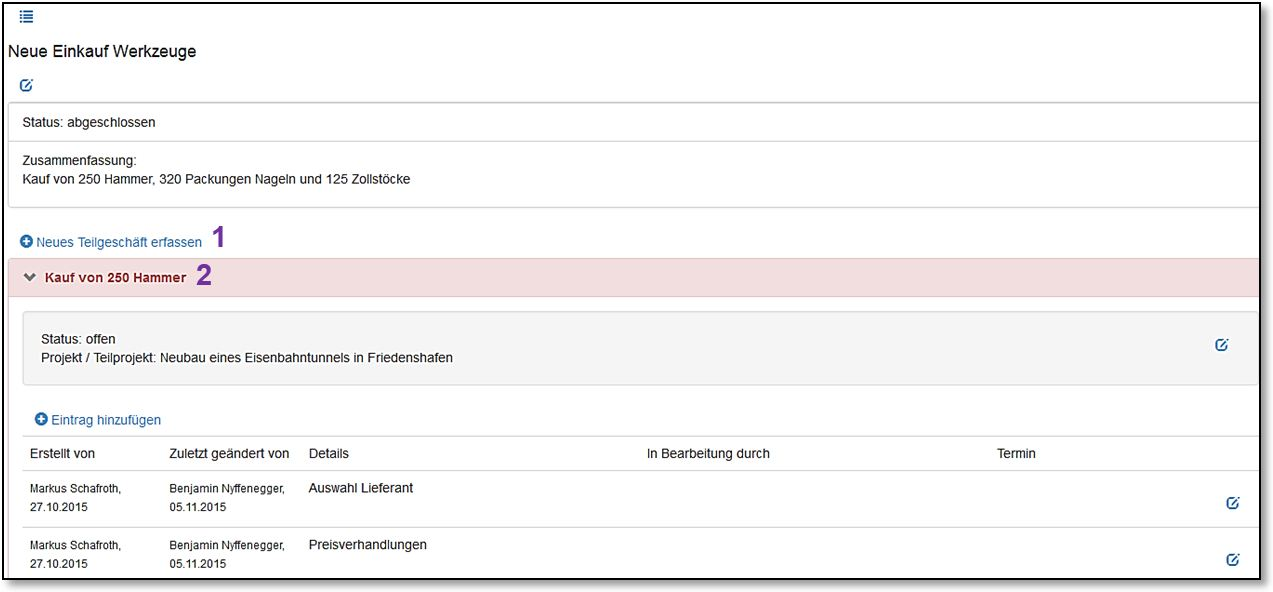
\includegraphics[width=1\linewidth]{../chapters/06_Geschaefte/pictures/6-2_GeschaefteUebersicht.jpg}}
\caption{Übersicht der Geschäfte}
% \label{fig:speciation}
\end{figure}

Unterhalb des Titels, des Status, der Zusammenfassung und der Beilagen finden Sie ein Pluszeichen 
\includegraphics[height=12pt]{../chapters/06_Geschaefte/pictures/6-2_TeilgeschaeftErfassen.jpg} \col{(1)} mit der Aufforderung zum Erfassen eines neuen Teilgeschäfts. Schon existierende Teilgeschäfte sind darunter dargestellt \col{(2)}.

\vspace{\baselineskip}

Klicken Sie auf 'Neues Teilgeschäft Erfassen' und es öffnet sich ein Fenster, in dem Sie die Angaben zum Teilgeschäft eintragen können.

\begin{figure}[H]
\center{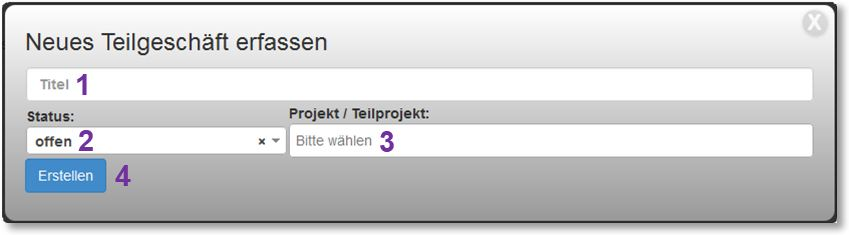
\includegraphics[width=0.5\linewidth]{../chapters/06_Geschaefte/pictures/6-2_NeuesTeilgeschaeftErfassen.jpg}}
\caption{Neues Teilgeschäft erfassen}
% \label{fig:speciation}
\end{figure}

Tragen Sie die erforderlichen Angaben in die Felder ein:

\begin{itemize}
\item
'Titel' \col{(1)} erlaubt die Eingabe von freiem Text.
\item
'Status' \col{(2)} ist automatisch auf 'offen' gesetzt, wenn das Teilgeschäft erledigt ist, können Sie den Status auf 'abgeschlossen' setzen.
\item
Das Feld 'Projekt/Teilprojekt' \col{(3)} enthält eine Auswahlliste, mit der Sie das Teilgeschäft mit einem Projekt oder Teilprojekt verknüpfen können. Das dem Teilgeschäft übergeordnete Geschäft erbt diese Verknüpfung, sie ist in der Liste der Geschäfte dargestellt. Das Geschäft erbt dann die Summe aller in den Teilgeschäften zugeordneten (Teil-)Projekte.
\end{itemize}

Klicken Sie auf die Schaltfläche 'Erstellen' \col{(4)} um das Teilgeschäft zu speichern. Der Titel des Teilgeschäfts erscheint nun in einem rosa Balken in der Übersicht des Geschäfts. Sie haben nun die Möglichkeit, entweder einen Eintrag zum neuen Teilgeschäft zu erfassen oder ein weiteres Teilgeschäft zu erstellen. Falls Sie mehrere Teilgeschäfte erfassen, erscheint in der Übersicht das zuletzt erfasste zuoberst.

\subsection{Den Überblick über ein Geschäft herstellen}

Möchten Sie den vollständigen Überblick über ein Geschäft erhalten, wählen Sie im Menü den Punkt 'Geschäfte'. In der Liste der Geschäfte können Sie das Geschäft suchen, zu dem Sie den Überblick benötigen.

\begin{figure}[H]
\center{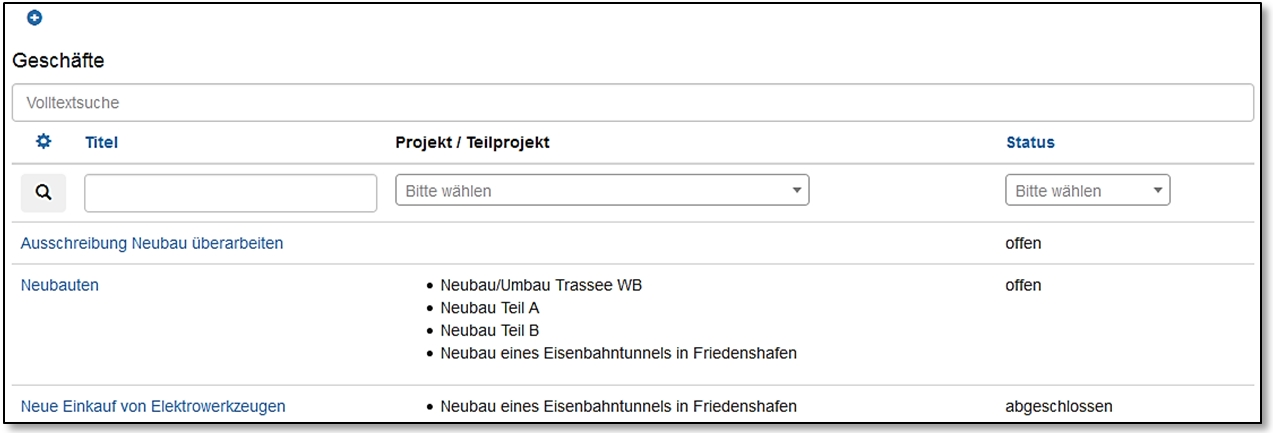
\includegraphics[width=1\linewidth]{../chapters/06_Geschaefte/pictures/6-3_UeberblickGeschaeft.jpg}}
\caption{Überblick über Geschäfte}
% \label{fig:speciation}
\end{figure}

Sie können nun optisch innerhalb der gesamten Liste der Geschäfte suchen oder die Liste filtern. Zum Blättern in der Liste scrollen Sie einfach nach unten, zuunterst sehen Sie Schaltflächen zum Blättern auf eine nächste Seite, oder zum Weiter- oder Zurückblättern.

\begin{center}

\includegraphics[height=12pt]{/Icons/SeitenBlaettern.jpg}
\end{center}

Zum Filtern der Liste stehen ihnen verschiedene Suchfelder zur Verfügung. Im Feld 'Titel' \col{(1)} können Sie freien Text eingeben; im Feld 'Projekt/Teilprojekt' \col{(2)}, sowie im Feld 'Status' \col{(3)} steht jeweils eine Auswahlliste zur Verfügung. Haben Sie die Filterwerte ausgewählt, klicken Sie auf das Lupensymbol 
\includegraphics[height=12pt]{/Icons/Lupe_kl.jpg} \col{(4)} links (oder drücken die 'Enter'-Taste) und die gefilterte Liste erscheint.

\begin{figure}[H]
\center{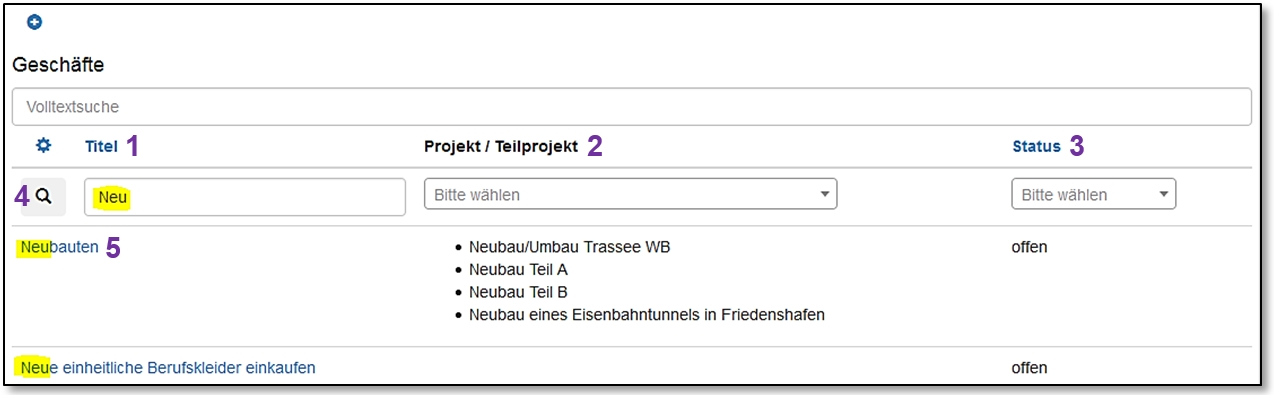
\includegraphics[width=1\linewidth]{../chapters/06_Geschaefte/pictures/6-3_GeschaefteFiltern.jpg}}
\caption{Geschäfte filtern}
% \label{fig:speciation}
\end{figure}

Haben sie das relevante Geschäft gefunden, klicken Sie auf den blauen Titeltext des entsprechenden Geschäfts \col{(5)}. Nun erscheint die Maske mit der Übersicht über das Geschäft.

\begin{figure}[H]
\center{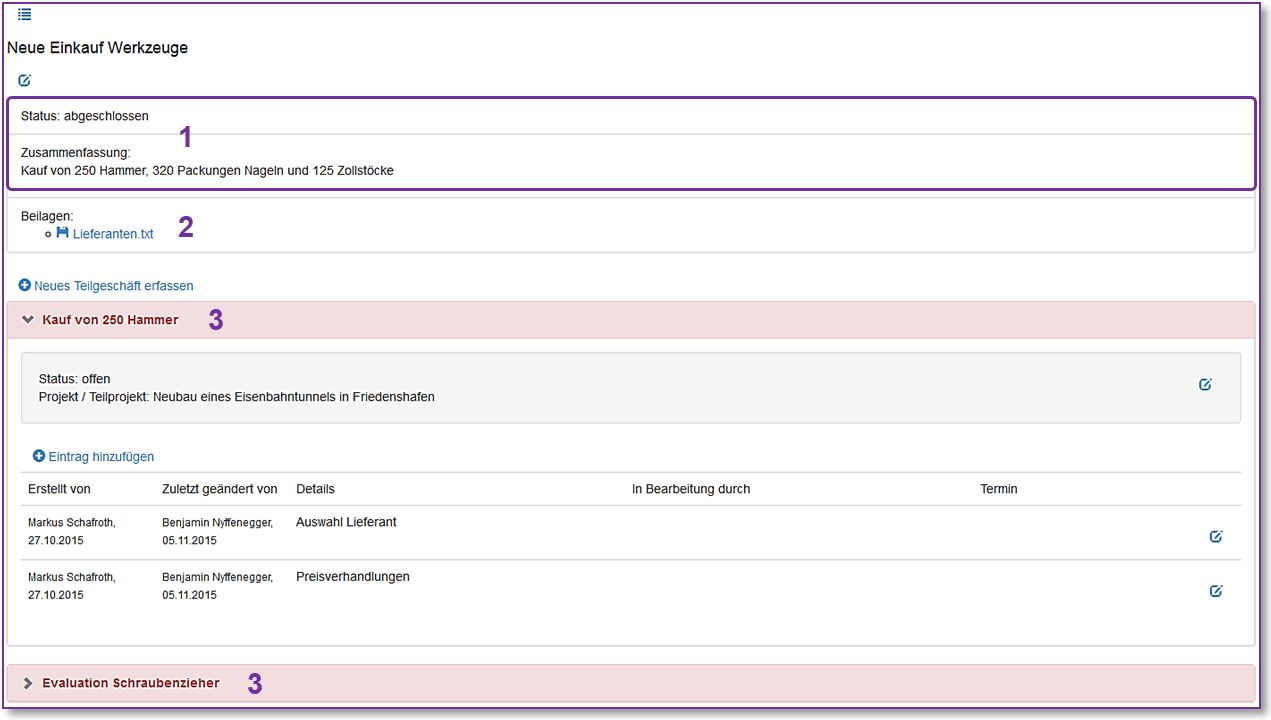
\includegraphics[width=1\linewidth]{../chapters/06_Geschaefte/pictures/6-3_Geschaeftsuebersicht.jpg}}
\caption{Übersicht des Geschäfts}
% \label{fig:speciation}
\end{figure}

In dieser Übersicht finden Sie oben die allgemeinen Informationen zum Geschäft \col{(1)} und darunter die Liste der Beilagen \col{(2)}, sofern solche erfasst wurden. Mit Klick auf den blauen Dateinamen können Sie die Beilagen herunterladen. Wurden mehrere Beilagen erfasst, können Sie diese mit Klick auf das ZIP-Symbol 
\includegraphics[height=12pt]{/Icons/ZIPSymbol.jpg} \col{(3)} zusammengefasst als ZIP-Datei herunterladen. Wiederum darunter sind die Teilgeschäfte aufgelistet \col{(4)}, mit jedem Titel in einem rosa Balken.

\vspace{\baselineskip}

Wählen Sie ein Teilgeschäft aus, und klicken Sie auf den Pfeil 
\includegraphics[height=12pt]{/Icons/Pfeil_rechts_rosa.jpg} links vom Titel. Dessen Richtung wechselt nun von seitlich auf senkrecht 
\includegraphics[height=12pt]{/Icons/Pfeil_unten_rosa.jpg} und die Inhalte des Teilgeschäfts erscheinen nun ausgeklappt. Oben finden Sie die allgemeinen Informationen zum Teilgeschäft, darunter die Einträge mit den jüngsten Einträgen zuoberst.

\vspace{\baselineskip}

Wiederholen Sie dies für alle Teilgeschäfte, und Sie haben den Überblick über alle Einträge zu allen Teilgeschäften eines Geschäfts.

\begin{figure}[H]
\center{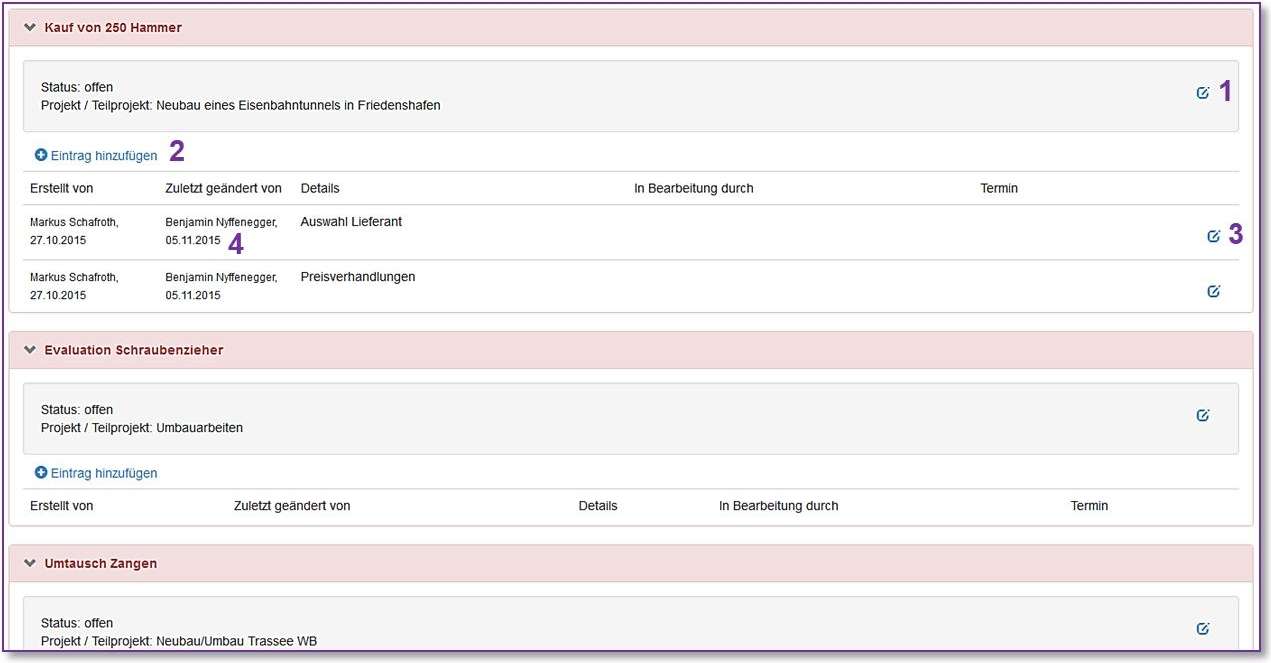
\includegraphics[width=1\linewidth]{../chapters/06_Geschaefte/pictures/6-3_UeberblickTeilgeschaefte.jpg}}
\caption{Überblick über die Teilgeschäfte}
% \label{fig:speciation}
\end{figure}

Das Bleistiftsymbol 
\includegraphics[height=12pt]{/Icons/Bearbeiten.jpg} \col{(1)} rechts der allgemeinen Informationen eines Teilgeschäfts ermöglicht Ihnen, diese zu überarbeiten.

\subsection{Einträge in Teilgeschäften hinzufügen}

Sie können einen Eintrag in einem Teilgeschäft entweder direkt nach dem Erfassen des Teilgeschäfts vornehmen oder jederzeit später, indem Sie wie im vorherigen Abschnitt beschrieben das Teilgeschäft suchen und den Inhalt anzeigen lassen.

Klicken Sie unter dem grauen Feld mit den allgemeinen Angaben zum Teilgeschäft auf 'Eintrag hinzufügen' 
\includegraphics[height=12pt]{../chapters/06_Geschaefte/pictures/6-4_TeilgeschaefteEintragHinzufuegen.jpg} \col{(1)}. Es erscheint das Fenster zum Erfassen von Einträgen.

\begin{figure}[H]
\center{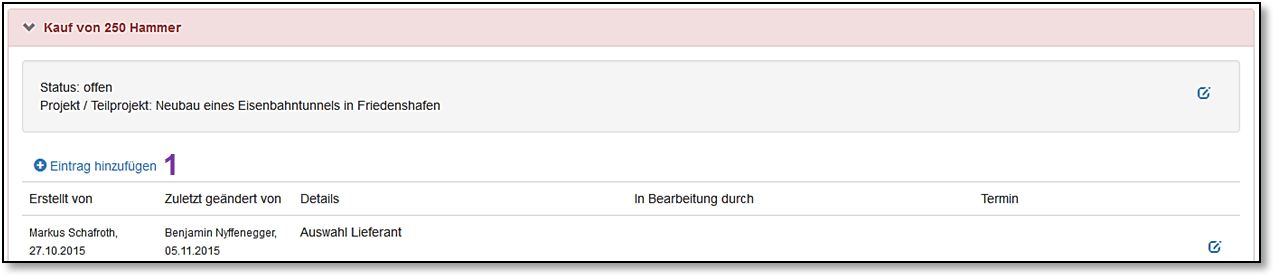
\includegraphics[width=1\linewidth]{../chapters/06_Geschaefte/pictures/6-4_TeilgeschaefteEintragHinzufuegenMaske.jpg}}
\caption{Übersicht des Teilgeschäftes}
% \label{fig:speciation}
\end{figure}

\begin{figure}[H]
\center{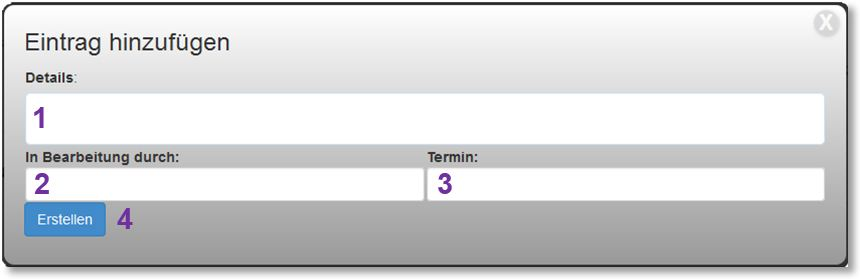
\includegraphics[width=.75\linewidth]{../chapters/06_Geschaefte/pictures/6-4_TeilgeschaefteHinzufuegenFelder.jpg}}
\caption{Eintrag in Teilgeschäft hinzufügen}
% \label{fig:speciation}
\end{figure}

Füllen Sie die Felder aus:

\begin{itemize}
\item
'Details' \col{(1)} enthält freien Text, der den Inhalt
des Eintrags beschreibt, z.B. die Beschreibung eines Vorgangs.
\item
'In Bearbeitung durch' \col{(2)} enthält freien Text, mit dem Sie angeben können, wer die im Eintrag beschriebene Angelegenheit bearbeitet.
\item
'Termin' \col{(3)} ist im Datumsformat TT.MM.JJJJ. auszufüllen. Hiermit können Sie angeben, bis wann die im Eintrag beschriebene Angelegenheit zu erledigen ist.
\item
Falls der Eintrag z.B. nur eine Feststellung beschreibt, ist es nicht erforderlich, die Felder 'In Bearbeitung durch' und 'Termin' auszufüllen.
\end{itemize}

Klicken Sie auf die Schaltfläche 'Erstellen' \col{(4)} und der Eintrag erscheint in der Übersicht des Teilgeschäfts.

\begin{figure}[H]
\center{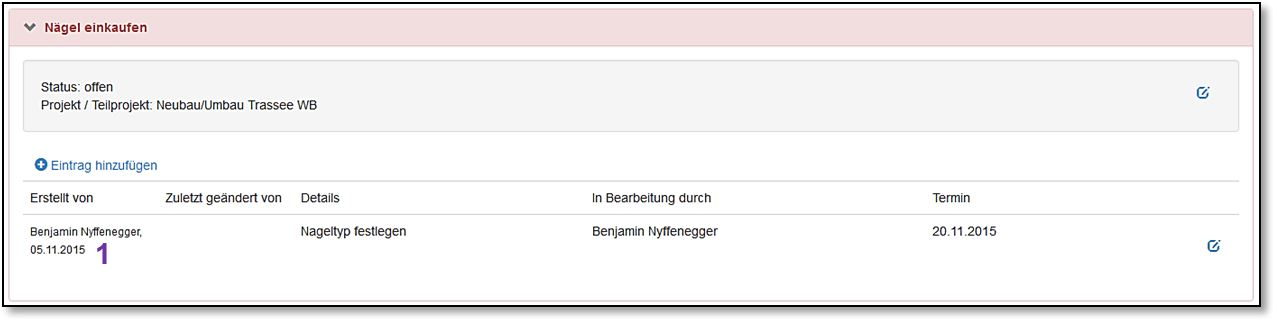
\includegraphics[width=1\linewidth]{../chapters/06_Geschaefte/pictures/6-4_TeilgeschaeftErstellen.jpg}}
\caption{Übersicht Teilgeschäft}
% \label{fig:speciation}
\end{figure}

Links des Eintrags sind das Datum der Erstellung und der Ersteller \col{(1)} ersichtlich. Dies soll dem Leser des Eintrags ermöglichen, den Eintrag zeitlich einzuordnen und Rückfragen betreffend des Eintrags vorzunehmen.

Sobald mehrere Einträge zu einem Teilgeschäft vorliegen, erscheinen diese in zeitlich absteigender Reihenfolge (jüngster Eintrag zuoberst).

\subsection{Bestehende Einträge überarbeiten}

Um einen bestehenden Eintrag zu überarbeiten, schaffen Sie sich zuerst wie oben beschrieben die Übersicht über das relevante Geschäft und seine Teilgeschäfte. Klappen Sie den Inhalt des Teilgeschäfts durch Klicken auf den Pfeil 
\includegraphics[height=12pt]{/Icons/Pfeil_rechts_rosa.jpg} links neben dem Titel aus.
	
\begin{figure}[H]
\center{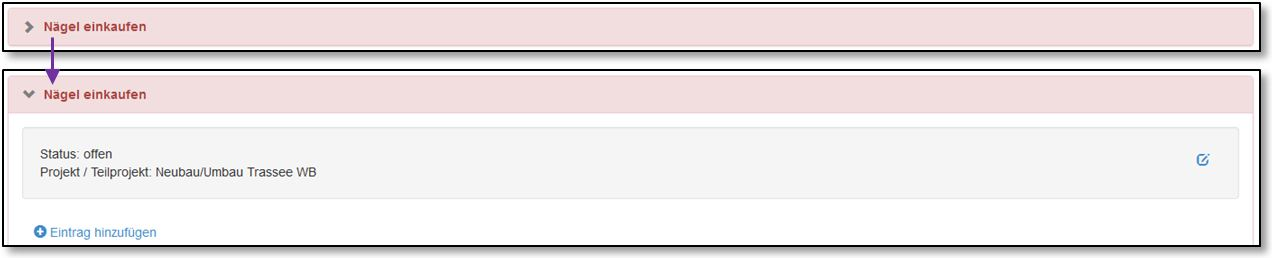
\includegraphics[width=1\linewidth]{../chapters/06_Geschaefte/pictures/6-5_GeschaefteDetails.jpg}}
\caption{Teilgeschäfte: Details anzeigen}
% \label{fig:speciation}
\end{figure}

Nun erscheinen alle Einträge in zeitlich absteigender Reihenfolge (jüngster Eintrag zuoberst).

\begin{figure}[H]
\center{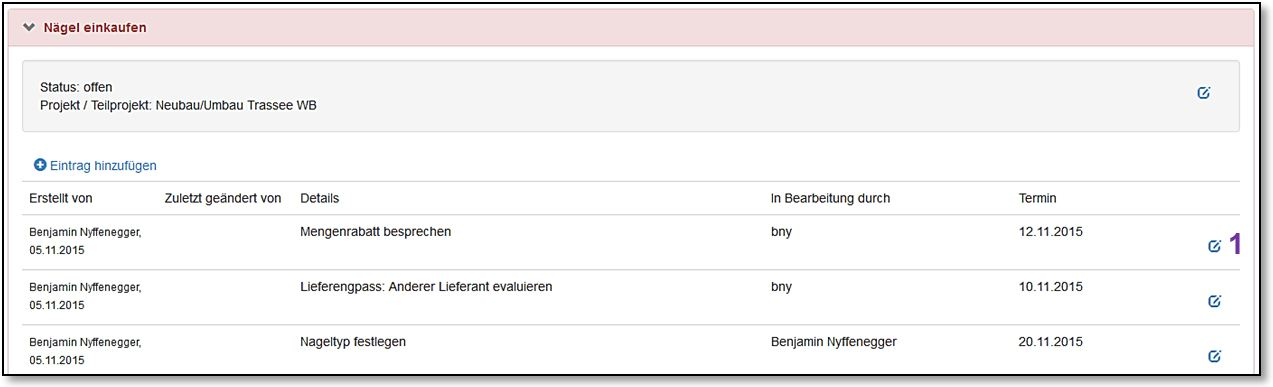
\includegraphics[width=1\linewidth]{../chapters/06_Geschaefte/pictures/6-5_GeschaefteEintraege.jpg}}
\caption{Teilgeschäfte: Alle Einträge anzeigen}
% \label{fig:speciation}
\end{figure}

Scrollen Sie durch die Einträge bis Sie den gewünschten Eintrag finden.

\vspace{\baselineskip}

Klicken Sie auf das Bleistiftsymbol 
\includegraphics[height=12pt]{/Icons/Bearbeiten.jpg} \col{(1)} rechts im Eintrag und es erscheint das Fenster zum Bearbeiten des Eintrags.

\begin{figure}[H]
\center{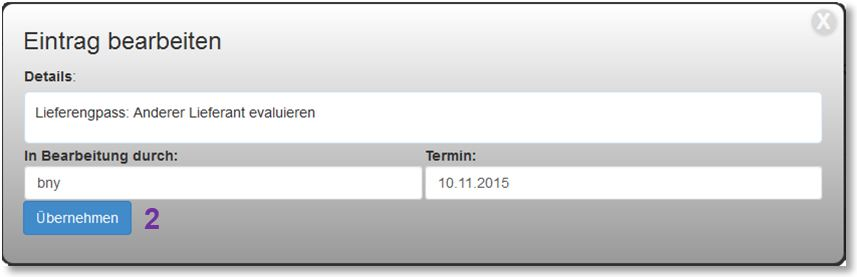
\includegraphics[width=.75\linewidth]{../chapters/06_Geschaefte/pictures/6-5_GeschaefteEintraegeBearbeiten.jpg}}
\caption{Teilgeschäfte: Einträge bearbeiten}
% \label{fig:speciation}
\end{figure}

Nehmen Sie in den Feldern Ihre Änderungen vor und klicken Sie auf 'Übernehmen' \col{(2)}. Nun erscheint der geänderte Eintrag in der Liste der Einträge. Links erscheint neben dem Datum der Erstellung und dem Ersteller auch das Datum der Änderung und wer die Änderung vorgenommen hat \col{(3)}.

\begin{figure}[H]
\center{
\includegraphics[width=1\linewidth]{../chapters/06_Geschaefte/pictures/6-5_GeschaefteEintraegeNachverf.jpg}}
\caption{Teilgeschäfte: Änderungen rückverfolgen}
% \label{fig:speciation}
\end{figure}

\textbf{Hinweis}: Der Inhalt der Änderungen wird nicht protokolliert, d.h. es ist nur der letzte Zustand der Feldinhalte gespeichert.

\vspace{\baselineskip}

\textbf{Hinweis}: Wenn ein Eintrag mehrmals verändert wird, bleiben nur das Datum der Erstellung, der Name des Erstellers, das Datum der letzten Änderung und der Name der Person, die die letzten Änderungen vorgenommen hat, gespeichert. Angaben zu den zwischenzeitlich vorgenommenen Änderungen gehen verloren.

\subsection{Allgemeine Angaben zu Geschäften überarbeiten}

Wählen Sie im Menü den Punkt 'Geschäfte' und suchen Sie in der Liste der Geschäfte das relevante Geschäft, entweder indem Sie optisch in der Liste suchen oder indem Sie die Liste filtern. Klicken Sie auf den blauen Titel des gewünschten Geschäfts. Das Geschäft wird mit der Detailanzeige geöffnet:

\begin{figure}[H]
\center{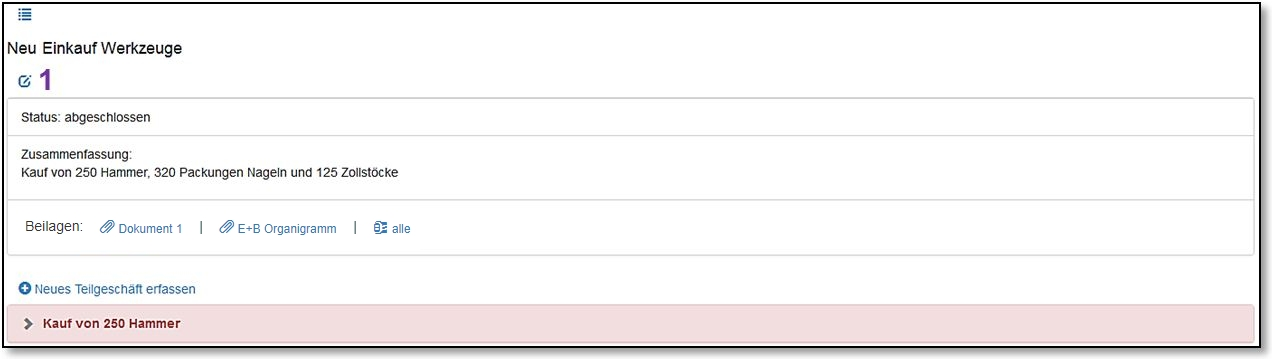
\includegraphics[width=1\linewidth]{../chapters/06_Geschaefte/pictures/6-6_GeschaefteEintragUeberblick.jpg}}
\caption{Geschäft Übersicht}
% \label{fig:speciation}
\end{figure}

Klicken Sie auf das Bleistiftsymbol 
\includegraphics[height=12pt]{/Icons/Bearbeiten.jpg} \col{(1)} unter dem Titel des Geschäfts.

\begin{figure}[H]
\center{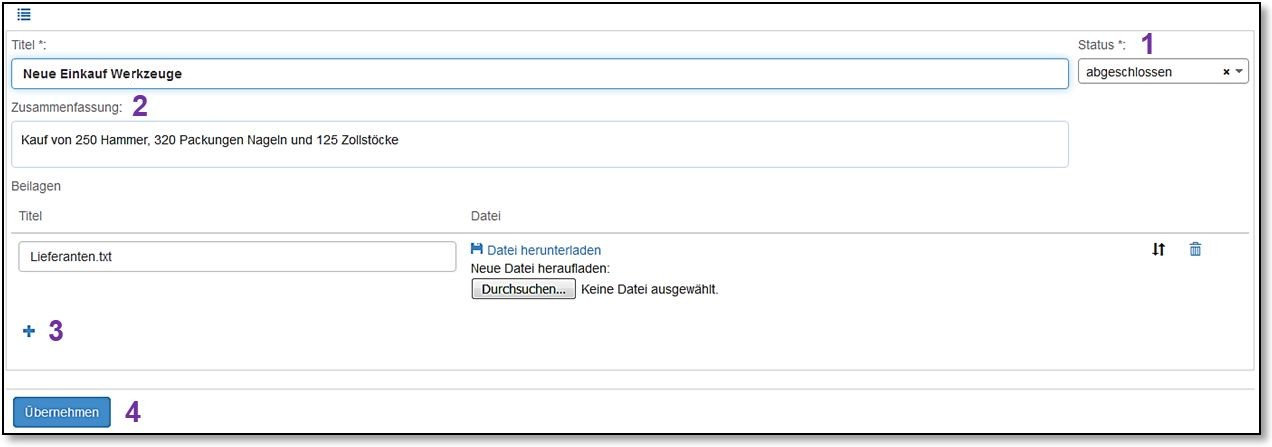
\includegraphics[width=1\linewidth]{../chapters/06_Geschaefte/pictures/6-6_GeschaefteEintragBearbeiten.jpg}}
\caption{Geschäft bearbeiten}
% \label{fig:speciation}
\end{figure}

Nun können Sie die Inhalte der Felder 'Status' \col{(1)} und 'Zusammenfassung' \col{(2)} bearbeiten, sowie neue Beilagen \col{(3)} verknüpfen oder hochladen. Klicken Sie auf 'Übernehmen', \col{(4)} um die Daten zu sichern oder auf 'Übernehmen und schliessen' (oben im Bildschirm), um nach dem Speichern zur Übersicht zurückzukehren.

\subsection{Allgemeine Angaben zu Teilgeschäften überarbeiten}

Verschaffen Sie sich wie oben beschrieben die Übersicht über das relevante Geschäft und die zugehörigen Teilgeschäfte. Klappen Sie den Inhalt des Teilgeschäfts durch Klicken auf den Pfeil 
\includegraphics[height=12pt]{/Icons/Pfeil_rechts_rosa.jpg} links neben dem Titel aus. Unter dem Titel erscheint ein graues Feld \col{(1)} mit den allgemeinen Inhalten zum Teilgeschäft.

\begin{figure}[H]
\center{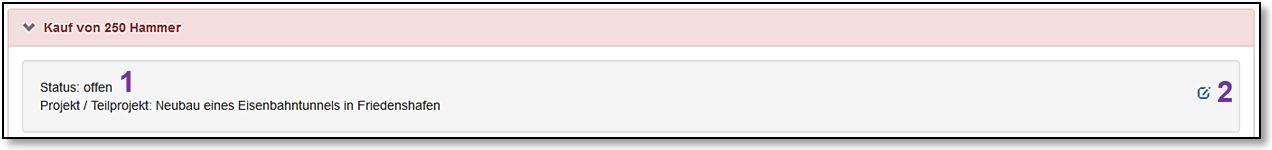
\includegraphics[width=1\linewidth]{../chapters/06_Geschaefte/pictures/6-7_Teilgeschaeft.jpg}}
\caption{Teilgeschäft Übersicht}
% \label{fig:speciation}
\end{figure}

Klicken Sie auf das Bleistiftsymbol 
\includegraphics[height=12pt]{/Icons/Bearbeiten.jpg} \col{(2)} rechts in diesem Feld. Es erscheint das Fenster zum Bearbeiten der allgemeinen Angaben des Teilgeschäfts.

\begin{figure}[H]
\center{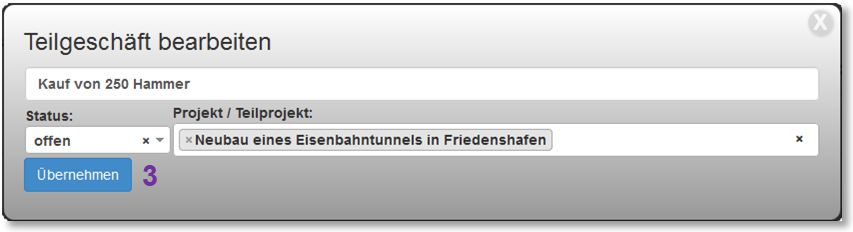
\includegraphics[width=.75\linewidth]{../chapters/06_Geschaefte/pictures/6-7_TeilgeschaeftBearbeiten.jpg}}
\caption{Teilgeschäft bearbeiten}
% \label{fig:speciation}
\end{figure}

Sie können nun die Inhalte der Felder überarbeiten. Klicken Sie auf 'Übernehmen' \col{(3)}, um die Daten zu sichern.
